% Created by tikzDevice version 0.7.0 on 2014-07-24 03:37:30
% !TEX encoding = UTF-8 Unicode
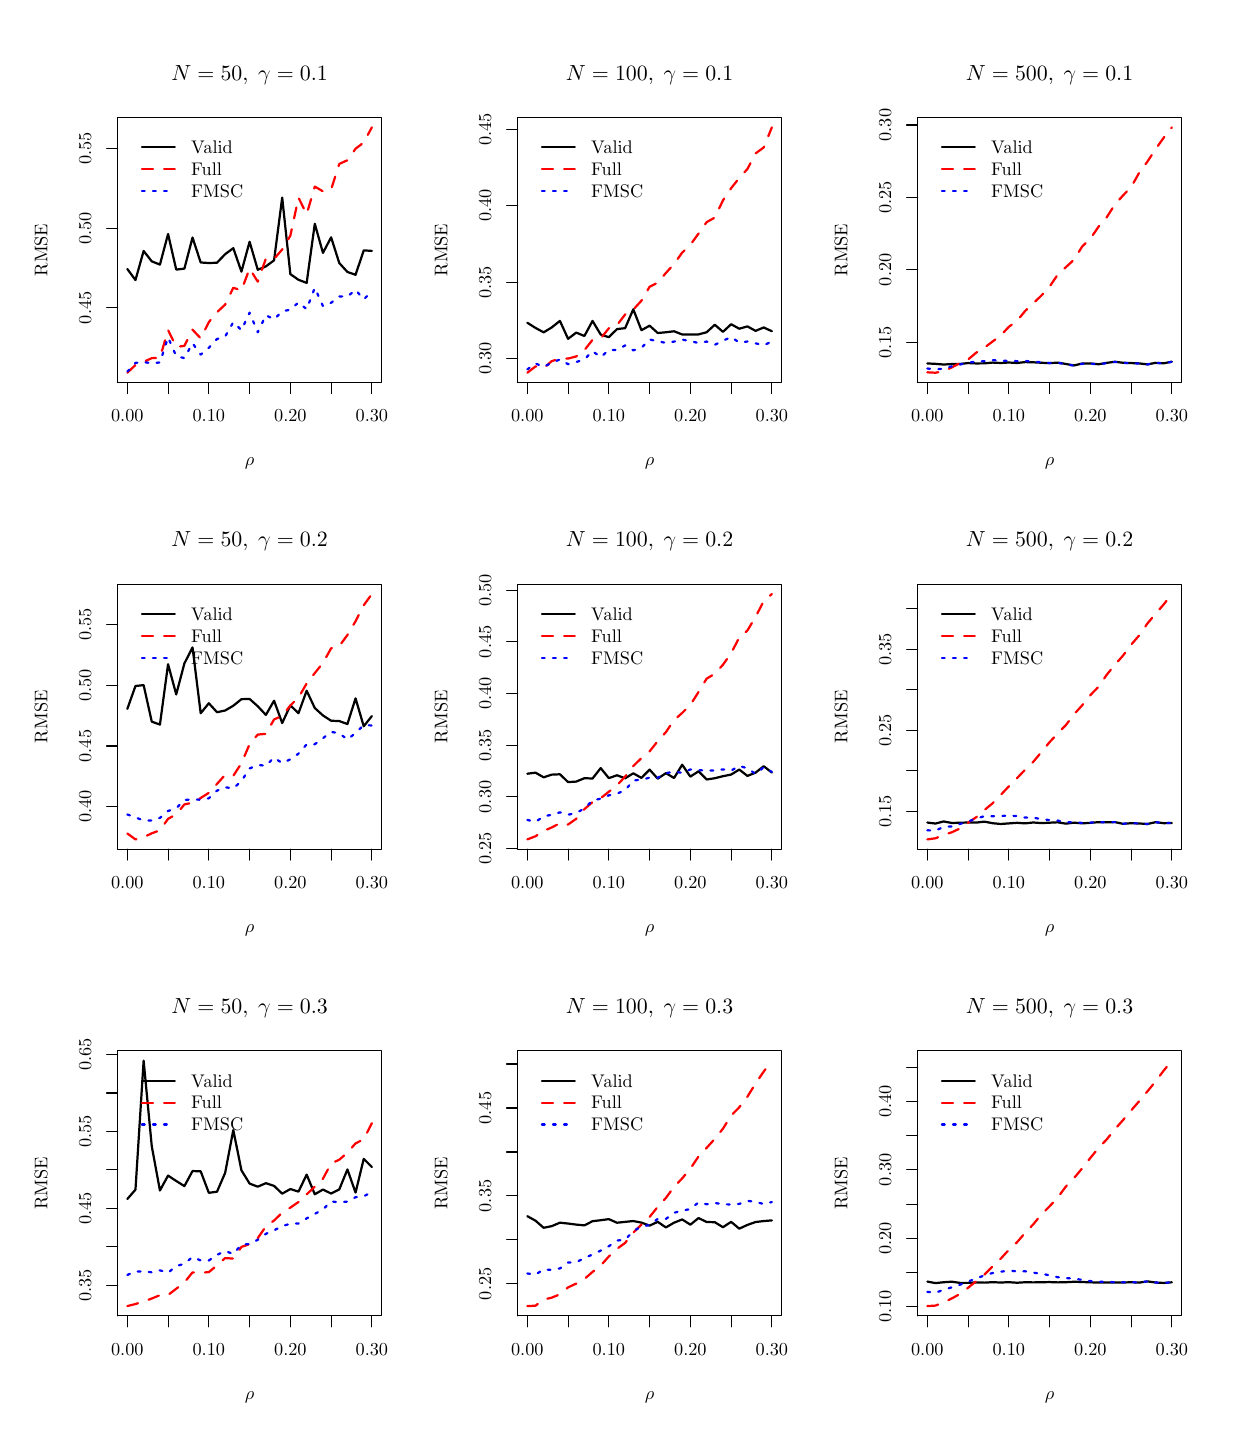
\begin{tikzpicture}[x=1pt,y=1pt]
\definecolor[named]{fillColor}{rgb}{1.00,1.00,1.00}
\path[use as bounding box,fill=fillColor,fill opacity=0.00] (0,0) rectangle (433.62,505.89);
\begin{scope}
\path[clip] ( 32.47,377.65) rectangle (127.91,473.42);
\definecolor[named]{drawColor}{rgb}{0.00,0.00,0.00}

\path[draw=drawColor,line width= 0.8pt,line join=round,line cap=round] ( 36.01,418.69) --
	( 38.95,414.69) --
	( 41.90,425.20) --
	( 44.84,421.44) --
	( 47.79,420.27) --
	( 50.73,431.33) --
	( 53.68,418.46) --
	( 56.63,418.82) --
	( 59.57,430.05) --
	( 62.52,421.04) --
	( 65.46,420.84) --
	( 68.41,420.95) --
	( 71.35,424.03) --
	( 74.30,426.21) --
	( 77.24,417.72) --
	( 80.19,428.53) --
	( 83.14,418.41) --
	( 86.08,419.63) --
	( 89.03,421.82) --
	( 91.97,444.48) --
	( 94.92,416.83) --
	( 97.86,414.78) --
	(100.81,413.66) --
	(103.75,435.03) --
	(106.70,424.50) --
	(109.65,430.12) --
	(112.59,420.84) --
	(115.54,417.61) --
	(118.48,416.59) --
	(121.43,425.41) --
	(124.37,425.22);
\end{scope}
\begin{scope}
\path[clip] (  0.00,  0.00) rectangle (433.62,505.89);
\definecolor[named]{drawColor}{rgb}{0.00,0.00,0.00}

\path[draw=drawColor,line width= 0.4pt,line join=round,line cap=round] ( 36.01,377.65) -- (124.37,377.65);

\path[draw=drawColor,line width= 0.4pt,line join=round,line cap=round] ( 36.01,377.65) -- ( 36.01,373.69);

\path[draw=drawColor,line width= 0.4pt,line join=round,line cap=round] ( 50.73,377.65) -- ( 50.73,373.69);

\path[draw=drawColor,line width= 0.4pt,line join=round,line cap=round] ( 65.46,377.65) -- ( 65.46,373.69);

\path[draw=drawColor,line width= 0.4pt,line join=round,line cap=round] ( 80.19,377.65) -- ( 80.19,373.69);

\path[draw=drawColor,line width= 0.4pt,line join=round,line cap=round] ( 94.92,377.65) -- ( 94.92,373.69);

\path[draw=drawColor,line width= 0.4pt,line join=round,line cap=round] (109.65,377.65) -- (109.65,373.69);

\path[draw=drawColor,line width= 0.4pt,line join=round,line cap=round] (124.37,377.65) -- (124.37,373.69);

\node[text=drawColor,anchor=base,inner sep=0pt, outer sep=0pt, scale=  0.66] at ( 36.01,363.40) {0.00};

\node[text=drawColor,anchor=base,inner sep=0pt, outer sep=0pt, scale=  0.66] at ( 65.46,363.40) {0.10};

\node[text=drawColor,anchor=base,inner sep=0pt, outer sep=0pt, scale=  0.66] at ( 94.92,363.40) {0.20};

\node[text=drawColor,anchor=base,inner sep=0pt, outer sep=0pt, scale=  0.66] at (124.37,363.40) {0.30};

\path[draw=drawColor,line width= 0.4pt,line join=round,line cap=round] ( 32.47,404.64) -- ( 32.47,462.22);

\path[draw=drawColor,line width= 0.4pt,line join=round,line cap=round] ( 32.47,404.64) -- ( 28.51,404.64);

\path[draw=drawColor,line width= 0.4pt,line join=round,line cap=round] ( 32.47,433.43) -- ( 28.51,433.43);

\path[draw=drawColor,line width= 0.4pt,line join=round,line cap=round] ( 32.47,462.22) -- ( 28.51,462.22);

\node[text=drawColor,rotate= 90.00,anchor=base,inner sep=0pt, outer sep=0pt, scale=  0.66] at ( 22.97,404.64) {0.45};

\node[text=drawColor,rotate= 90.00,anchor=base,inner sep=0pt, outer sep=0pt, scale=  0.66] at ( 22.97,433.43) {0.50};

\node[text=drawColor,rotate= 90.00,anchor=base,inner sep=0pt, outer sep=0pt, scale=  0.66] at ( 22.97,462.22) {0.55};

\path[draw=drawColor,line width= 0.4pt,line join=round,line cap=round] ( 32.47,377.65) --
	(127.91,377.65) --
	(127.91,473.42) --
	( 32.47,473.42) --
	( 32.47,377.65);
\end{scope}
\begin{scope}
\path[clip] (  0.00,337.26) rectangle (144.54,505.89);
\definecolor[named]{drawColor}{rgb}{0.00,0.00,0.00}

\node[text=drawColor,anchor=base,inner sep=0pt, outer sep=0pt, scale=  0.79] at ( 80.19,486.92) {\bfseries $N=50, \;\gamma=0.1$};

\node[text=drawColor,anchor=base,inner sep=0pt, outer sep=0pt, scale=  0.66] at ( 80.19,347.56) {$\rho$};

\node[text=drawColor,rotate= 90.00,anchor=base,inner sep=0pt, outer sep=0pt, scale=  0.66] at (  7.13,425.53) {RMSE};
\end{scope}
\begin{scope}
\path[clip] ( 32.47,377.65) rectangle (127.91,473.42);
\definecolor[named]{drawColor}{rgb}{1.00,0.00,0.00}

\path[draw=drawColor,line width= 0.8pt,dash pattern=on 4pt off 4pt ,line join=round,line cap=round] ( 36.01,381.20) --
	( 38.95,383.98) --
	( 41.90,385.12) --
	( 44.84,386.47) --
	( 47.79,386.59) --
	( 50.73,396.61) --
	( 53.68,390.53) --
	( 56.63,390.90) --
	( 59.57,396.76) --
	( 62.52,393.63) --
	( 65.46,399.48) --
	( 68.41,403.05) --
	( 71.35,405.82) --
	( 74.30,411.89) --
	( 77.24,410.96) --
	( 80.19,418.86) --
	( 83.14,414.10) --
	( 86.08,422.44) --
	( 89.03,422.32) --
	( 91.97,425.73) --
	( 94.92,430.74) --
	( 97.86,444.45) --
	(100.81,438.47) --
	(103.75,448.47) --
	(106.70,446.74) --
	(109.65,447.44) --
	(112.59,456.64) --
	(115.54,457.98) --
	(118.48,462.14) --
	(121.43,464.40) --
	(124.37,469.87);
\definecolor[named]{drawColor}{rgb}{0.00,0.00,1.00}

\path[draw=drawColor,line width= 0.8pt,dash pattern=on 1pt off 3pt ,line join=round,line cap=round] ( 36.01,381.60) --
	( 38.95,384.76) --
	( 41.90,385.05) --
	( 44.84,384.61) --
	( 47.79,384.91) --
	( 50.73,393.97) --
	( 53.68,387.18) --
	( 56.63,386.49) --
	( 59.57,391.86) --
	( 62.52,387.76) --
	( 65.46,390.21) --
	( 68.41,393.39) --
	( 71.35,394.27) --
	( 74.30,399.48) --
	( 77.24,396.60) --
	( 80.19,402.92) --
	( 83.14,395.81) --
	( 86.08,401.99) --
	( 89.03,400.46) --
	( 91.97,403.42) --
	( 94.92,403.97) --
	( 97.86,406.62) --
	(100.81,404.14) --
	(103.75,411.88) --
	(106.70,405.27) --
	(109.65,406.47) --
	(112.59,408.78) --
	(115.54,408.71) --
	(118.48,411.16) --
	(121.43,407.67) --
	(124.37,410.73);
\definecolor[named]{drawColor}{rgb}{0.00,0.00,0.00}

\path[draw=drawColor,line width= 0.8pt,line join=round,line cap=round] ( 41.28,462.63) -- ( 53.16,462.63);
\definecolor[named]{drawColor}{rgb}{1.00,0.00,0.00}

\path[draw=drawColor,line width= 0.8pt,dash pattern=on 4pt off 4pt ,line join=round,line cap=round] ( 41.28,454.71) -- ( 53.16,454.71);
\definecolor[named]{drawColor}{rgb}{0.00,0.00,1.00}

\path[draw=drawColor,line width= 0.8pt,dash pattern=on 1pt off 3pt ,line join=round,line cap=round] ( 41.28,446.79) -- ( 53.16,446.79);
\definecolor[named]{drawColor}{rgb}{0.00,0.00,0.00}

\node[text=drawColor,anchor=base west,inner sep=0pt, outer sep=0pt, scale=  0.66] at ( 59.10,460.35) {Valid};

\node[text=drawColor,anchor=base west,inner sep=0pt, outer sep=0pt, scale=  0.66] at ( 59.10,452.43) {Full};

\node[text=drawColor,anchor=base west,inner sep=0pt, outer sep=0pt, scale=  0.66] at ( 59.10,444.51) {FMSC};
\end{scope}
\begin{scope}
\path[clip] (177.01,377.65) rectangle (272.45,473.42);
\definecolor[named]{drawColor}{rgb}{0.00,0.00,0.00}

\path[draw=drawColor,line width= 0.8pt,line join=round,line cap=round] (180.55,399.25) --
	(183.49,397.40) --
	(186.44,395.79) --
	(189.38,397.57) --
	(192.33,399.92) --
	(195.27,393.45) --
	(198.22,395.70) --
	(201.17,394.47) --
	(204.11,399.93) --
	(207.06,394.99) --
	(210.00,394.04) --
	(212.95,396.97) --
	(215.89,397.30) --
	(218.84,404.12) --
	(221.78,396.56) --
	(224.73,398.21) --
	(227.68,395.55) --
	(230.62,395.82) --
	(233.57,396.18) --
	(236.51,395.02) --
	(239.46,395.05) --
	(242.40,395.05) --
	(245.35,395.83) --
	(248.29,398.54) --
	(251.24,395.97) --
	(254.19,398.73) --
	(257.13,397.10) --
	(260.08,397.94) --
	(263.02,396.33) --
	(265.97,397.55) --
	(268.91,396.20);
\end{scope}
\begin{scope}
\path[clip] (  0.00,  0.00) rectangle (433.62,505.89);
\definecolor[named]{drawColor}{rgb}{0.00,0.00,0.00}

\path[draw=drawColor,line width= 0.4pt,line join=round,line cap=round] (180.55,377.65) -- (268.91,377.65);

\path[draw=drawColor,line width= 0.4pt,line join=round,line cap=round] (180.55,377.65) -- (180.55,373.69);

\path[draw=drawColor,line width= 0.4pt,line join=round,line cap=round] (195.27,377.65) -- (195.27,373.69);

\path[draw=drawColor,line width= 0.4pt,line join=round,line cap=round] (210.00,377.65) -- (210.00,373.69);

\path[draw=drawColor,line width= 0.4pt,line join=round,line cap=round] (224.73,377.65) -- (224.73,373.69);

\path[draw=drawColor,line width= 0.4pt,line join=round,line cap=round] (239.46,377.65) -- (239.46,373.69);

\path[draw=drawColor,line width= 0.4pt,line join=round,line cap=round] (254.19,377.65) -- (254.19,373.69);

\path[draw=drawColor,line width= 0.4pt,line join=round,line cap=round] (268.91,377.65) -- (268.91,373.69);

\node[text=drawColor,anchor=base,inner sep=0pt, outer sep=0pt, scale=  0.66] at (180.55,363.40) {0.00};

\node[text=drawColor,anchor=base,inner sep=0pt, outer sep=0pt, scale=  0.66] at (210.00,363.40) {0.10};

\node[text=drawColor,anchor=base,inner sep=0pt, outer sep=0pt, scale=  0.66] at (239.46,363.40) {0.20};

\node[text=drawColor,anchor=base,inner sep=0pt, outer sep=0pt, scale=  0.66] at (268.91,363.40) {0.30};

\path[draw=drawColor,line width= 0.4pt,line join=round,line cap=round] (177.01,386.28) -- (177.01,469.19);

\path[draw=drawColor,line width= 0.4pt,line join=round,line cap=round] (177.01,386.28) -- (173.05,386.28);

\path[draw=drawColor,line width= 0.4pt,line join=round,line cap=round] (177.01,413.92) -- (173.05,413.92);

\path[draw=drawColor,line width= 0.4pt,line join=round,line cap=round] (177.01,441.56) -- (173.05,441.56);

\path[draw=drawColor,line width= 0.4pt,line join=round,line cap=round] (177.01,469.19) -- (173.05,469.19);

\node[text=drawColor,rotate= 90.00,anchor=base,inner sep=0pt, outer sep=0pt, scale=  0.66] at (167.51,386.28) {0.30};

\node[text=drawColor,rotate= 90.00,anchor=base,inner sep=0pt, outer sep=0pt, scale=  0.66] at (167.51,413.92) {0.35};

\node[text=drawColor,rotate= 90.00,anchor=base,inner sep=0pt, outer sep=0pt, scale=  0.66] at (167.51,441.56) {0.40};

\node[text=drawColor,rotate= 90.00,anchor=base,inner sep=0pt, outer sep=0pt, scale=  0.66] at (167.51,469.19) {0.45};

\path[draw=drawColor,line width= 0.4pt,line join=round,line cap=round] (177.01,377.65) --
	(272.45,377.65) --
	(272.45,473.42) --
	(177.01,473.42) --
	(177.01,377.65);
\end{scope}
\begin{scope}
\path[clip] (144.54,337.26) rectangle (289.08,505.89);
\definecolor[named]{drawColor}{rgb}{0.00,0.00,0.00}

\node[text=drawColor,anchor=base,inner sep=0pt, outer sep=0pt, scale=  0.79] at (224.73,486.92) {\bfseries $N=100, \;\gamma=0.1$};

\node[text=drawColor,anchor=base,inner sep=0pt, outer sep=0pt, scale=  0.66] at (224.73,347.56) {$\rho$};

\node[text=drawColor,rotate= 90.00,anchor=base,inner sep=0pt, outer sep=0pt, scale=  0.66] at (151.67,425.53) {RMSE};
\end{scope}
\begin{scope}
\path[clip] (177.01,377.65) rectangle (272.45,473.42);
\definecolor[named]{drawColor}{rgb}{1.00,0.00,0.00}

\path[draw=drawColor,line width= 0.8pt,dash pattern=on 4pt off 4pt ,line join=round,line cap=round] (180.55,381.20) --
	(183.49,383.47) --
	(186.44,382.84) --
	(189.38,385.41) --
	(192.33,386.25) --
	(195.27,386.32) --
	(198.22,387.09) --
	(201.17,389.34) --
	(204.11,393.09) --
	(207.06,393.60) --
	(210.00,397.25) --
	(212.95,398.38) --
	(215.89,402.26) --
	(218.84,404.03) --
	(221.78,407.22) --
	(224.73,412.27) --
	(227.68,413.76) --
	(230.62,417.24) --
	(233.57,420.51) --
	(236.51,424.61) --
	(239.46,427.43) --
	(242.40,431.46) --
	(245.35,435.62) --
	(248.29,437.26) --
	(251.24,443.48) --
	(254.19,447.88) --
	(257.13,451.57) --
	(260.08,454.82) --
	(263.02,460.45) --
	(265.97,462.60) --
	(268.91,469.87);
\definecolor[named]{drawColor}{rgb}{0.00,0.00,1.00}

\path[draw=drawColor,line width= 0.8pt,dash pattern=on 1pt off 3pt ,line join=round,line cap=round] (180.55,382.41) --
	(183.49,384.56) --
	(186.44,383.30) --
	(189.38,384.82) --
	(192.33,386.00) --
	(195.27,384.28) --
	(198.22,385.07) --
	(201.17,386.01) --
	(204.11,388.98) --
	(207.06,386.84) --
	(210.00,389.39) --
	(212.95,389.44) --
	(215.89,391.06) --
	(218.84,389.30) --
	(221.78,390.20) --
	(224.73,393.21) --
	(227.68,392.55) --
	(230.62,391.99) --
	(233.57,392.44) --
	(236.51,393.17) --
	(239.46,392.63) --
	(242.40,391.93) --
	(245.35,392.47) --
	(248.29,391.30) --
	(251.24,392.74) --
	(254.19,394.12) --
	(257.13,392.09) --
	(260.08,392.47) --
	(263.02,391.83) --
	(265.97,391.14) --
	(268.91,392.47);
\definecolor[named]{drawColor}{rgb}{0.00,0.00,0.00}

\path[draw=drawColor,line width= 0.8pt,line join=round,line cap=round] (185.82,462.63) -- (197.70,462.63);
\definecolor[named]{drawColor}{rgb}{1.00,0.00,0.00}

\path[draw=drawColor,line width= 0.8pt,dash pattern=on 4pt off 4pt ,line join=round,line cap=round] (185.82,454.71) -- (197.70,454.71);
\definecolor[named]{drawColor}{rgb}{0.00,0.00,1.00}

\path[draw=drawColor,line width= 0.8pt,dash pattern=on 1pt off 3pt ,line join=round,line cap=round] (185.82,446.79) -- (197.70,446.79);
\definecolor[named]{drawColor}{rgb}{0.00,0.00,0.00}

\node[text=drawColor,anchor=base west,inner sep=0pt, outer sep=0pt, scale=  0.66] at (203.64,460.35) {Valid};

\node[text=drawColor,anchor=base west,inner sep=0pt, outer sep=0pt, scale=  0.66] at (203.64,452.43) {Full};

\node[text=drawColor,anchor=base west,inner sep=0pt, outer sep=0pt, scale=  0.66] at (203.64,444.51) {FMSC};
\end{scope}
\begin{scope}
\path[clip] (321.55,377.65) rectangle (416.99,473.42);
\definecolor[named]{drawColor}{rgb}{0.00,0.00,0.00}

\path[draw=drawColor,line width= 0.8pt,line join=round,line cap=round] (325.09,384.56) --
	(328.03,384.40) --
	(330.98,384.16) --
	(333.92,384.33) --
	(336.87,384.38) --
	(339.81,384.69) --
	(342.76,384.56) --
	(345.71,384.59) --
	(348.65,384.86) --
	(351.60,384.72) --
	(354.54,384.89) --
	(357.49,384.72) --
	(360.43,385.04) --
	(363.38,384.97) --
	(366.32,384.80) --
	(369.27,384.66) --
	(372.22,384.85) --
	(375.16,384.36) --
	(378.11,383.83) --
	(381.05,384.54) --
	(384.00,384.55) --
	(386.94,384.26) --
	(389.89,384.76) --
	(392.83,385.16) --
	(395.78,384.80) --
	(398.73,384.69) --
	(401.67,384.57) --
	(404.62,384.21) --
	(407.56,384.77) --
	(410.51,384.61) --
	(413.45,385.19);
\end{scope}
\begin{scope}
\path[clip] (  0.00,  0.00) rectangle (433.62,505.89);
\definecolor[named]{drawColor}{rgb}{0.00,0.00,0.00}

\path[draw=drawColor,line width= 0.4pt,line join=round,line cap=round] (325.09,377.65) -- (413.45,377.65);

\path[draw=drawColor,line width= 0.4pt,line join=round,line cap=round] (325.09,377.65) -- (325.09,373.69);

\path[draw=drawColor,line width= 0.4pt,line join=round,line cap=round] (339.81,377.65) -- (339.81,373.69);

\path[draw=drawColor,line width= 0.4pt,line join=round,line cap=round] (354.54,377.65) -- (354.54,373.69);

\path[draw=drawColor,line width= 0.4pt,line join=round,line cap=round] (369.27,377.65) -- (369.27,373.69);

\path[draw=drawColor,line width= 0.4pt,line join=round,line cap=round] (384.00,377.65) -- (384.00,373.69);

\path[draw=drawColor,line width= 0.4pt,line join=round,line cap=round] (398.73,377.65) -- (398.73,373.69);

\path[draw=drawColor,line width= 0.4pt,line join=round,line cap=round] (413.45,377.65) -- (413.45,373.69);

\node[text=drawColor,anchor=base,inner sep=0pt, outer sep=0pt, scale=  0.66] at (325.09,363.40) {0.00};

\node[text=drawColor,anchor=base,inner sep=0pt, outer sep=0pt, scale=  0.66] at (354.54,363.40) {0.10};

\node[text=drawColor,anchor=base,inner sep=0pt, outer sep=0pt, scale=  0.66] at (384.00,363.40) {0.20};

\node[text=drawColor,anchor=base,inner sep=0pt, outer sep=0pt, scale=  0.66] at (413.45,363.40) {0.30};

\path[draw=drawColor,line width= 0.4pt,line join=round,line cap=round] (321.55,392.24) -- (321.55,470.71);

\path[draw=drawColor,line width= 0.4pt,line join=round,line cap=round] (321.55,392.24) -- (317.59,392.24);

\path[draw=drawColor,line width= 0.4pt,line join=round,line cap=round] (321.55,418.40) -- (317.59,418.40);

\path[draw=drawColor,line width= 0.4pt,line join=round,line cap=round] (321.55,444.55) -- (317.59,444.55);

\path[draw=drawColor,line width= 0.4pt,line join=round,line cap=round] (321.55,470.71) -- (317.59,470.71);

\node[text=drawColor,rotate= 90.00,anchor=base,inner sep=0pt, outer sep=0pt, scale=  0.66] at (312.05,392.24) {0.15};

\node[text=drawColor,rotate= 90.00,anchor=base,inner sep=0pt, outer sep=0pt, scale=  0.66] at (312.05,418.40) {0.20};

\node[text=drawColor,rotate= 90.00,anchor=base,inner sep=0pt, outer sep=0pt, scale=  0.66] at (312.05,444.55) {0.25};

\node[text=drawColor,rotate= 90.00,anchor=base,inner sep=0pt, outer sep=0pt, scale=  0.66] at (312.05,470.71) {0.30};

\path[draw=drawColor,line width= 0.4pt,line join=round,line cap=round] (321.55,377.65) --
	(416.99,377.65) --
	(416.99,473.42) --
	(321.55,473.42) --
	(321.55,377.65);
\end{scope}
\begin{scope}
\path[clip] (289.08,337.26) rectangle (433.62,505.89);
\definecolor[named]{drawColor}{rgb}{0.00,0.00,0.00}

\node[text=drawColor,anchor=base,inner sep=0pt, outer sep=0pt, scale=  0.79] at (369.27,486.92) {\bfseries $N=500, \;\gamma=0.1$};

\node[text=drawColor,anchor=base,inner sep=0pt, outer sep=0pt, scale=  0.66] at (369.27,347.56) {$\rho$};

\node[text=drawColor,rotate= 90.00,anchor=base,inner sep=0pt, outer sep=0pt, scale=  0.66] at (296.21,425.53) {RMSE};
\end{scope}
\begin{scope}
\path[clip] (321.55,377.65) rectangle (416.99,473.42);
\definecolor[named]{drawColor}{rgb}{1.00,0.00,0.00}

\path[draw=drawColor,line width= 0.8pt,dash pattern=on 4pt off 4pt ,line join=round,line cap=round] (325.09,381.35) --
	(328.03,381.20) --
	(330.98,381.75) --
	(333.92,383.12) --
	(336.87,384.68) --
	(339.81,385.98) --
	(342.76,388.46) --
	(345.71,390.26) --
	(348.65,392.47) --
	(351.60,394.65) --
	(354.54,397.79) --
	(357.49,399.92) --
	(360.43,403.51) --
	(363.38,406.29) --
	(366.32,409.11) --
	(369.27,412.33) --
	(372.22,416.68) --
	(375.16,419.34) --
	(378.11,422.07) --
	(381.05,426.83) --
	(384.00,429.63) --
	(386.94,433.95) --
	(389.89,437.33) --
	(392.83,441.97) --
	(395.78,445.24) --
	(398.73,448.26) --
	(401.67,453.52) --
	(404.62,457.49) --
	(407.56,461.99) --
	(410.51,466.12) --
	(413.45,469.87);
\definecolor[named]{drawColor}{rgb}{0.00,0.00,1.00}

\path[draw=drawColor,line width= 0.8pt,dash pattern=on 1pt off 3pt ,line join=round,line cap=round] (325.09,382.72) --
	(328.03,382.47) --
	(330.98,382.65) --
	(333.92,383.52) --
	(336.87,384.16) --
	(339.81,384.84) --
	(342.76,385.20) --
	(345.71,385.39) --
	(348.65,385.75) --
	(351.60,385.55) --
	(354.54,385.46) --
	(357.49,385.39) --
	(360.43,385.43) --
	(363.38,385.26) --
	(366.32,384.96) --
	(369.27,384.68) --
	(372.22,384.79) --
	(375.16,384.28) --
	(378.11,383.74) --
	(381.05,384.42) --
	(384.00,384.50) --
	(386.94,384.21) --
	(389.89,384.69) --
	(392.83,385.11) --
	(395.78,384.77) --
	(398.73,384.65) --
	(401.67,384.52) --
	(404.62,384.19) --
	(407.56,384.74) --
	(410.51,384.57) --
	(413.45,385.16);
\definecolor[named]{drawColor}{rgb}{0.00,0.00,0.00}

\path[draw=drawColor,line width= 0.8pt,line join=round,line cap=round] (330.36,462.63) -- (342.24,462.63);
\definecolor[named]{drawColor}{rgb}{1.00,0.00,0.00}

\path[draw=drawColor,line width= 0.8pt,dash pattern=on 4pt off 4pt ,line join=round,line cap=round] (330.36,454.71) -- (342.24,454.71);
\definecolor[named]{drawColor}{rgb}{0.00,0.00,1.00}

\path[draw=drawColor,line width= 0.8pt,dash pattern=on 1pt off 3pt ,line join=round,line cap=round] (330.36,446.79) -- (342.24,446.79);
\definecolor[named]{drawColor}{rgb}{0.00,0.00,0.00}

\node[text=drawColor,anchor=base west,inner sep=0pt, outer sep=0pt, scale=  0.66] at (348.18,460.35) {Valid};

\node[text=drawColor,anchor=base west,inner sep=0pt, outer sep=0pt, scale=  0.66] at (348.18,452.43) {Full};

\node[text=drawColor,anchor=base west,inner sep=0pt, outer sep=0pt, scale=  0.66] at (348.18,444.51) {FMSC};
\end{scope}
\begin{scope}
\path[clip] ( 32.47,209.02) rectangle (127.91,304.79);
\definecolor[named]{drawColor}{rgb}{0.00,0.00,0.00}

\path[draw=drawColor,line width= 0.8pt,line join=round,line cap=round] ( 36.01,259.74) --
	( 38.95,268.00) --
	( 41.90,268.32) --
	( 44.84,255.12) --
	( 47.79,254.06) --
	( 50.73,275.88) --
	( 53.68,264.96) --
	( 56.63,276.16) --
	( 59.57,281.94) --
	( 62.52,258.15) --
	( 65.46,261.77) --
	( 68.41,258.53) --
	( 71.35,259.14) --
	( 74.30,260.87) --
	( 77.24,263.24) --
	( 80.19,263.32) --
	( 83.14,260.68) --
	( 86.08,257.55) --
	( 89.03,262.69) --
	( 91.97,254.61) --
	( 94.92,261.00) --
	( 97.86,258.17) --
	(100.81,266.29) --
	(103.75,260.04) --
	(106.70,257.35) --
	(109.65,255.45) --
	(112.59,255.33) --
	(115.54,254.26) --
	(118.48,263.53) --
	(121.43,253.45) --
	(124.37,257.13);
\end{scope}
\begin{scope}
\path[clip] (  0.00,  0.00) rectangle (433.62,505.89);
\definecolor[named]{drawColor}{rgb}{0.00,0.00,0.00}

\path[draw=drawColor,line width= 0.4pt,line join=round,line cap=round] ( 36.01,209.02) -- (124.37,209.02);

\path[draw=drawColor,line width= 0.4pt,line join=round,line cap=round] ( 36.01,209.02) -- ( 36.01,205.06);

\path[draw=drawColor,line width= 0.4pt,line join=round,line cap=round] ( 50.73,209.02) -- ( 50.73,205.06);

\path[draw=drawColor,line width= 0.4pt,line join=round,line cap=round] ( 65.46,209.02) -- ( 65.46,205.06);

\path[draw=drawColor,line width= 0.4pt,line join=round,line cap=round] ( 80.19,209.02) -- ( 80.19,205.06);

\path[draw=drawColor,line width= 0.4pt,line join=round,line cap=round] ( 94.92,209.02) -- ( 94.92,205.06);

\path[draw=drawColor,line width= 0.4pt,line join=round,line cap=round] (109.65,209.02) -- (109.65,205.06);

\path[draw=drawColor,line width= 0.4pt,line join=round,line cap=round] (124.37,209.02) -- (124.37,205.06);

\node[text=drawColor,anchor=base,inner sep=0pt, outer sep=0pt, scale=  0.66] at ( 36.01,194.77) {0.00};

\node[text=drawColor,anchor=base,inner sep=0pt, outer sep=0pt, scale=  0.66] at ( 65.46,194.77) {0.10};

\node[text=drawColor,anchor=base,inner sep=0pt, outer sep=0pt, scale=  0.66] at ( 94.92,194.77) {0.20};

\node[text=drawColor,anchor=base,inner sep=0pt, outer sep=0pt, scale=  0.66] at (124.37,194.77) {0.30};

\path[draw=drawColor,line width= 0.4pt,line join=round,line cap=round] ( 32.47,224.37) -- ( 32.47,290.24);

\path[draw=drawColor,line width= 0.4pt,line join=round,line cap=round] ( 32.47,224.37) -- ( 28.51,224.37);

\path[draw=drawColor,line width= 0.4pt,line join=round,line cap=round] ( 32.47,246.33) -- ( 28.51,246.33);

\path[draw=drawColor,line width= 0.4pt,line join=round,line cap=round] ( 32.47,268.28) -- ( 28.51,268.28);

\path[draw=drawColor,line width= 0.4pt,line join=round,line cap=round] ( 32.47,290.24) -- ( 28.51,290.24);

\node[text=drawColor,rotate= 90.00,anchor=base,inner sep=0pt, outer sep=0pt, scale=  0.66] at ( 22.97,224.37) {0.40};

\node[text=drawColor,rotate= 90.00,anchor=base,inner sep=0pt, outer sep=0pt, scale=  0.66] at ( 22.97,246.33) {0.45};

\node[text=drawColor,rotate= 90.00,anchor=base,inner sep=0pt, outer sep=0pt, scale=  0.66] at ( 22.97,268.28) {0.50};

\node[text=drawColor,rotate= 90.00,anchor=base,inner sep=0pt, outer sep=0pt, scale=  0.66] at ( 22.97,290.24) {0.55};

\path[draw=drawColor,line width= 0.4pt,line join=round,line cap=round] ( 32.47,209.02) --
	(127.91,209.02) --
	(127.91,304.79) --
	( 32.47,304.79) --
	( 32.47,209.02);
\end{scope}
\begin{scope}
\path[clip] (  0.00,168.63) rectangle (144.54,337.26);
\definecolor[named]{drawColor}{rgb}{0.00,0.00,0.00}

\node[text=drawColor,anchor=base,inner sep=0pt, outer sep=0pt, scale=  0.79] at ( 80.19,318.29) {\bfseries $N=50, \;\gamma=0.2$};

\node[text=drawColor,anchor=base,inner sep=0pt, outer sep=0pt, scale=  0.66] at ( 80.19,178.93) {$\rho$};

\node[text=drawColor,rotate= 90.00,anchor=base,inner sep=0pt, outer sep=0pt, scale=  0.66] at (  7.13,256.90) {RMSE};
\end{scope}
\begin{scope}
\path[clip] ( 32.47,209.02) rectangle (127.91,304.79);
\definecolor[named]{drawColor}{rgb}{1.00,0.00,0.00}

\path[draw=drawColor,line width= 0.8pt,dash pattern=on 4pt off 4pt ,line join=round,line cap=round] ( 36.01,214.71) --
	( 38.95,212.57) --
	( 41.90,213.37) --
	( 44.84,214.77) --
	( 47.79,215.87) --
	( 50.73,220.01) --
	( 53.68,221.59) --
	( 56.63,225.21) --
	( 59.57,225.84) --
	( 62.52,227.53) --
	( 65.46,229.40) --
	( 68.41,232.63) --
	( 71.35,235.89) --
	( 74.30,235.56) --
	( 77.24,240.06) --
	( 80.19,247.00) --
	( 83.14,250.45) --
	( 86.08,250.71) --
	( 89.03,255.91) --
	( 91.97,257.23) --
	( 94.92,260.96) --
	( 97.86,263.82) --
	(100.81,268.91) --
	(103.75,272.66) --
	(106.70,276.35) --
	(109.65,281.62) --
	(112.59,282.41) --
	(115.54,286.42) --
	(118.48,291.41) --
	(121.43,297.17) --
	(124.37,301.24);
\definecolor[named]{drawColor}{rgb}{0.00,0.00,1.00}

\path[draw=drawColor,line width= 0.8pt,dash pattern=on 1pt off 3pt ,line join=round,line cap=round] ( 36.01,221.58) --
	( 38.95,220.51) --
	( 41.90,219.40) --
	( 44.84,219.40) --
	( 47.79,220.34) --
	( 50.73,222.84) --
	( 53.68,223.82) --
	( 56.63,226.80) --
	( 59.57,227.05) --
	( 62.52,226.90) --
	( 65.46,227.43) --
	( 68.41,230.17) --
	( 71.35,231.43) --
	( 74.30,230.97) --
	( 77.24,233.65) --
	( 80.19,238.19) --
	( 83.14,239.48) --
	( 86.08,239.19) --
	( 89.03,242.16) --
	( 91.97,240.10) --
	( 94.92,241.51) --
	( 97.86,243.55) --
	(100.81,246.90) --
	(103.75,246.95) --
	(106.70,249.14) --
	(109.65,251.39) --
	(112.59,250.99) --
	(115.54,248.62) --
	(118.48,251.06) --
	(121.43,253.84) --
	(124.37,253.75);
\definecolor[named]{drawColor}{rgb}{0.00,0.00,0.00}

\path[draw=drawColor,line width= 0.8pt,line join=round,line cap=round] ( 41.28,294.00) -- ( 53.16,294.00);
\definecolor[named]{drawColor}{rgb}{1.00,0.00,0.00}

\path[draw=drawColor,line width= 0.8pt,dash pattern=on 4pt off 4pt ,line join=round,line cap=round] ( 41.28,286.08) -- ( 53.16,286.08);
\definecolor[named]{drawColor}{rgb}{0.00,0.00,1.00}

\path[draw=drawColor,line width= 0.8pt,dash pattern=on 1pt off 3pt ,line join=round,line cap=round] ( 41.28,278.16) -- ( 53.16,278.16);
\definecolor[named]{drawColor}{rgb}{0.00,0.00,0.00}

\node[text=drawColor,anchor=base west,inner sep=0pt, outer sep=0pt, scale=  0.66] at ( 59.10,291.72) {Valid};

\node[text=drawColor,anchor=base west,inner sep=0pt, outer sep=0pt, scale=  0.66] at ( 59.10,283.80) {Full};

\node[text=drawColor,anchor=base west,inner sep=0pt, outer sep=0pt, scale=  0.66] at ( 59.10,275.88) {FMSC};
\end{scope}
\begin{scope}
\path[clip] (177.01,209.02) rectangle (272.45,304.79);
\definecolor[named]{drawColor}{rgb}{0.00,0.00,0.00}

\path[draw=drawColor,line width= 0.8pt,line join=round,line cap=round] (180.55,236.30) --
	(183.49,236.69) --
	(186.44,235.01) --
	(189.38,235.97) --
	(192.33,236.10) --
	(195.27,233.28) --
	(198.22,233.46) --
	(201.17,234.68) --
	(204.11,234.57) --
	(207.06,238.34) --
	(210.00,234.71) --
	(212.95,235.74) --
	(215.89,234.65) --
	(218.84,236.45) --
	(221.78,234.79) --
	(224.73,237.79) --
	(227.68,234.51) --
	(230.62,236.51) --
	(233.57,234.75) --
	(236.51,239.56) --
	(239.46,235.25) --
	(242.40,237.18) --
	(245.35,234.22) --
	(248.29,234.67) --
	(251.24,235.41) --
	(254.19,236.00) --
	(257.13,237.80) --
	(260.08,235.51) --
	(263.02,236.69) --
	(265.97,239.02) --
	(268.91,236.72);
\end{scope}
\begin{scope}
\path[clip] (  0.00,  0.00) rectangle (433.62,505.89);
\definecolor[named]{drawColor}{rgb}{0.00,0.00,0.00}

\path[draw=drawColor,line width= 0.4pt,line join=round,line cap=round] (180.55,209.02) -- (268.91,209.02);

\path[draw=drawColor,line width= 0.4pt,line join=round,line cap=round] (180.55,209.02) -- (180.55,205.06);

\path[draw=drawColor,line width= 0.4pt,line join=round,line cap=round] (195.27,209.02) -- (195.27,205.06);

\path[draw=drawColor,line width= 0.4pt,line join=round,line cap=round] (210.00,209.02) -- (210.00,205.06);

\path[draw=drawColor,line width= 0.4pt,line join=round,line cap=round] (224.73,209.02) -- (224.73,205.06);

\path[draw=drawColor,line width= 0.4pt,line join=round,line cap=round] (239.46,209.02) -- (239.46,205.06);

\path[draw=drawColor,line width= 0.4pt,line join=round,line cap=round] (254.19,209.02) -- (254.19,205.06);

\path[draw=drawColor,line width= 0.4pt,line join=round,line cap=round] (268.91,209.02) -- (268.91,205.06);

\node[text=drawColor,anchor=base,inner sep=0pt, outer sep=0pt, scale=  0.66] at (180.55,194.77) {0.00};

\node[text=drawColor,anchor=base,inner sep=0pt, outer sep=0pt, scale=  0.66] at (210.00,194.77) {0.10};

\node[text=drawColor,anchor=base,inner sep=0pt, outer sep=0pt, scale=  0.66] at (239.46,194.77) {0.20};

\node[text=drawColor,anchor=base,inner sep=0pt, outer sep=0pt, scale=  0.66] at (268.91,194.77) {0.30};

\path[draw=drawColor,line width= 0.4pt,line join=round,line cap=round] (177.01,209.25) -- (177.01,302.62);

\path[draw=drawColor,line width= 0.4pt,line join=round,line cap=round] (177.01,209.25) -- (173.05,209.25);

\path[draw=drawColor,line width= 0.4pt,line join=round,line cap=round] (177.01,227.92) -- (173.05,227.92);

\path[draw=drawColor,line width= 0.4pt,line join=round,line cap=round] (177.01,246.60) -- (173.05,246.60);

\path[draw=drawColor,line width= 0.4pt,line join=round,line cap=round] (177.01,265.27) -- (173.05,265.27);

\path[draw=drawColor,line width= 0.4pt,line join=round,line cap=round] (177.01,283.95) -- (173.05,283.95);

\path[draw=drawColor,line width= 0.4pt,line join=round,line cap=round] (177.01,302.62) -- (173.05,302.62);

\node[text=drawColor,rotate= 90.00,anchor=base,inner sep=0pt, outer sep=0pt, scale=  0.66] at (167.51,209.25) {0.25};

\node[text=drawColor,rotate= 90.00,anchor=base,inner sep=0pt, outer sep=0pt, scale=  0.66] at (167.51,227.92) {0.30};

\node[text=drawColor,rotate= 90.00,anchor=base,inner sep=0pt, outer sep=0pt, scale=  0.66] at (167.51,246.60) {0.35};

\node[text=drawColor,rotate= 90.00,anchor=base,inner sep=0pt, outer sep=0pt, scale=  0.66] at (167.51,265.27) {0.40};

\node[text=drawColor,rotate= 90.00,anchor=base,inner sep=0pt, outer sep=0pt, scale=  0.66] at (167.51,283.95) {0.45};

\node[text=drawColor,rotate= 90.00,anchor=base,inner sep=0pt, outer sep=0pt, scale=  0.66] at (167.51,302.62) {0.50};

\path[draw=drawColor,line width= 0.4pt,line join=round,line cap=round] (177.01,209.02) --
	(272.45,209.02) --
	(272.45,304.79) --
	(177.01,304.79) --
	(177.01,209.02);
\end{scope}
\begin{scope}
\path[clip] (144.54,168.63) rectangle (289.08,337.26);
\definecolor[named]{drawColor}{rgb}{0.00,0.00,0.00}

\node[text=drawColor,anchor=base,inner sep=0pt, outer sep=0pt, scale=  0.79] at (224.73,318.29) {\bfseries $N=100, \;\gamma=0.2$};

\node[text=drawColor,anchor=base,inner sep=0pt, outer sep=0pt, scale=  0.66] at (224.73,178.93) {$\rho$};

\node[text=drawColor,rotate= 90.00,anchor=base,inner sep=0pt, outer sep=0pt, scale=  0.66] at (151.67,256.90) {RMSE};
\end{scope}
\begin{scope}
\path[clip] (177.01,209.02) rectangle (272.45,304.79);
\definecolor[named]{drawColor}{rgb}{1.00,0.00,0.00}

\path[draw=drawColor,line width= 0.8pt,dash pattern=on 4pt off 4pt ,line join=round,line cap=round] (180.55,212.57) --
	(183.49,213.70) --
	(186.44,215.61) --
	(189.38,216.90) --
	(192.33,218.41) --
	(195.27,217.95) --
	(198.22,220.02) --
	(201.17,223.49) --
	(204.11,226.06) --
	(207.06,227.47) --
	(210.00,229.78) --
	(212.95,232.10) --
	(215.89,235.27) --
	(218.84,239.08) --
	(221.78,241.96) --
	(224.73,244.39) --
	(227.68,248.08) --
	(230.62,251.32) --
	(233.57,255.66) --
	(236.51,258.27) --
	(239.46,261.16) --
	(242.40,265.81) --
	(245.35,270.68) --
	(248.29,272.40) --
	(251.24,275.69) --
	(254.19,279.84) --
	(257.13,285.53) --
	(260.08,288.05) --
	(263.02,292.99) --
	(265.97,298.65) --
	(268.91,301.24);
\definecolor[named]{drawColor}{rgb}{0.00,0.00,1.00}

\path[draw=drawColor,line width= 0.8pt,dash pattern=on 1pt off 3pt ,line join=round,line cap=round] (180.55,219.61) --
	(183.49,218.89) --
	(186.44,220.89) --
	(189.38,221.47) --
	(192.33,222.35) --
	(195.27,221.48) --
	(198.22,222.12) --
	(201.17,223.74) --
	(204.11,226.65) --
	(207.06,227.29) --
	(210.00,228.49) --
	(212.95,229.13) --
	(215.89,230.29) --
	(218.84,233.88) --
	(221.78,234.14) --
	(224.73,234.86) --
	(227.68,234.87) --
	(230.62,236.52) --
	(233.57,237.02) --
	(236.51,236.63) --
	(239.46,237.84) --
	(242.40,237.57) --
	(245.35,237.51) --
	(248.29,237.43) --
	(251.24,237.87) --
	(254.19,237.43) --
	(257.13,239.13) --
	(260.08,238.25) --
	(263.02,236.24) --
	(265.97,238.62) --
	(268.91,236.97);
\definecolor[named]{drawColor}{rgb}{0.00,0.00,0.00}

\path[draw=drawColor,line width= 0.8pt,line join=round,line cap=round] (185.82,294.00) -- (197.70,294.00);
\definecolor[named]{drawColor}{rgb}{1.00,0.00,0.00}

\path[draw=drawColor,line width= 0.8pt,dash pattern=on 4pt off 4pt ,line join=round,line cap=round] (185.82,286.08) -- (197.70,286.08);
\definecolor[named]{drawColor}{rgb}{0.00,0.00,1.00}

\path[draw=drawColor,line width= 0.8pt,dash pattern=on 1pt off 3pt ,line join=round,line cap=round] (185.82,278.16) -- (197.70,278.16);
\definecolor[named]{drawColor}{rgb}{0.00,0.00,0.00}

\node[text=drawColor,anchor=base west,inner sep=0pt, outer sep=0pt, scale=  0.66] at (203.64,291.72) {Valid};

\node[text=drawColor,anchor=base west,inner sep=0pt, outer sep=0pt, scale=  0.66] at (203.64,283.80) {Full};

\node[text=drawColor,anchor=base west,inner sep=0pt, outer sep=0pt, scale=  0.66] at (203.64,275.88) {FMSC};
\end{scope}
\begin{scope}
\path[clip] (321.55,209.02) rectangle (416.99,304.79);
\definecolor[named]{drawColor}{rgb}{0.00,0.00,0.00}

\path[draw=drawColor,line width= 0.8pt,line join=round,line cap=round] (325.09,218.66) --
	(328.03,218.30) --
	(330.98,219.05) --
	(333.92,218.51) --
	(336.87,218.58) --
	(339.81,218.68) --
	(342.76,218.64) --
	(345.71,218.99) --
	(348.65,218.42) --
	(351.60,218.14) --
	(354.54,218.35) --
	(357.49,218.56) --
	(360.43,218.36) --
	(363.38,218.68) --
	(366.32,218.46) --
	(369.27,218.61) --
	(372.22,218.74) --
	(375.16,218.26) --
	(378.11,218.62) --
	(381.05,218.36) --
	(384.00,218.56) --
	(386.94,218.80) --
	(389.89,218.75) --
	(392.83,218.82) --
	(395.78,218.21) --
	(398.73,218.42) --
	(401.67,218.32) --
	(404.62,218.14) --
	(407.56,218.79) --
	(410.51,218.43) --
	(413.45,218.49);
\end{scope}
\begin{scope}
\path[clip] (  0.00,  0.00) rectangle (433.62,505.89);
\definecolor[named]{drawColor}{rgb}{0.00,0.00,0.00}

\path[draw=drawColor,line width= 0.4pt,line join=round,line cap=round] (325.09,209.02) -- (413.45,209.02);

\path[draw=drawColor,line width= 0.4pt,line join=round,line cap=round] (325.09,209.02) -- (325.09,205.06);

\path[draw=drawColor,line width= 0.4pt,line join=round,line cap=round] (339.81,209.02) -- (339.81,205.06);

\path[draw=drawColor,line width= 0.4pt,line join=round,line cap=round] (354.54,209.02) -- (354.54,205.06);

\path[draw=drawColor,line width= 0.4pt,line join=round,line cap=round] (369.27,209.02) -- (369.27,205.06);

\path[draw=drawColor,line width= 0.4pt,line join=round,line cap=round] (384.00,209.02) -- (384.00,205.06);

\path[draw=drawColor,line width= 0.4pt,line join=round,line cap=round] (398.73,209.02) -- (398.73,205.06);

\path[draw=drawColor,line width= 0.4pt,line join=round,line cap=round] (413.45,209.02) -- (413.45,205.06);

\node[text=drawColor,anchor=base,inner sep=0pt, outer sep=0pt, scale=  0.66] at (325.09,194.77) {0.00};

\node[text=drawColor,anchor=base,inner sep=0pt, outer sep=0pt, scale=  0.66] at (354.54,194.77) {0.10};

\node[text=drawColor,anchor=base,inner sep=0pt, outer sep=0pt, scale=  0.66] at (384.00,194.77) {0.20};

\node[text=drawColor,anchor=base,inner sep=0pt, outer sep=0pt, scale=  0.66] at (413.45,194.77) {0.30};

\path[draw=drawColor,line width= 0.4pt,line join=round,line cap=round] (321.55,222.75) -- (321.55,295.87);

\path[draw=drawColor,line width= 0.4pt,line join=round,line cap=round] (321.55,222.75) -- (317.59,222.75);

\path[draw=drawColor,line width= 0.4pt,line join=round,line cap=round] (321.55,237.38) -- (317.59,237.38);

\path[draw=drawColor,line width= 0.4pt,line join=round,line cap=round] (321.55,252.00) -- (317.59,252.00);

\path[draw=drawColor,line width= 0.4pt,line join=round,line cap=round] (321.55,266.63) -- (317.59,266.63);

\path[draw=drawColor,line width= 0.4pt,line join=round,line cap=round] (321.55,281.25) -- (317.59,281.25);

\path[draw=drawColor,line width= 0.4pt,line join=round,line cap=round] (321.55,295.87) -- (317.59,295.87);

\node[text=drawColor,rotate= 90.00,anchor=base,inner sep=0pt, outer sep=0pt, scale=  0.66] at (312.05,222.75) {0.15};

\node[text=drawColor,rotate= 90.00,anchor=base,inner sep=0pt, outer sep=0pt, scale=  0.66] at (312.05,252.00) {0.25};

\node[text=drawColor,rotate= 90.00,anchor=base,inner sep=0pt, outer sep=0pt, scale=  0.66] at (312.05,281.25) {0.35};

\path[draw=drawColor,line width= 0.4pt,line join=round,line cap=round] (321.55,209.02) --
	(416.99,209.02) --
	(416.99,304.79) --
	(321.55,304.79) --
	(321.55,209.02);
\end{scope}
\begin{scope}
\path[clip] (289.08,168.63) rectangle (433.62,337.26);
\definecolor[named]{drawColor}{rgb}{0.00,0.00,0.00}

\node[text=drawColor,anchor=base,inner sep=0pt, outer sep=0pt, scale=  0.79] at (369.27,318.29) {\bfseries $N=500, \;\gamma=0.2$};

\node[text=drawColor,anchor=base,inner sep=0pt, outer sep=0pt, scale=  0.66] at (369.27,178.93) {$\rho$};

\node[text=drawColor,rotate= 90.00,anchor=base,inner sep=0pt, outer sep=0pt, scale=  0.66] at (296.21,256.90) {RMSE};
\end{scope}
\begin{scope}
\path[clip] (321.55,209.02) rectangle (416.99,304.79);
\definecolor[named]{drawColor}{rgb}{1.00,0.00,0.00}

\path[draw=drawColor,line width= 0.8pt,dash pattern=on 4pt off 4pt ,line join=round,line cap=round] (325.09,212.57) --
	(328.03,212.97) --
	(330.98,214.19) --
	(333.92,215.13) --
	(336.87,216.51) --
	(339.81,218.61) --
	(342.76,220.59) --
	(345.71,223.18) --
	(348.65,225.59) --
	(351.60,228.63) --
	(354.54,231.74) --
	(357.49,234.70) --
	(360.43,237.77) --
	(363.38,240.61) --
	(366.32,244.15) --
	(369.27,247.72) --
	(372.22,250.87) --
	(375.16,253.89) --
	(378.11,257.79) --
	(381.05,261.03) --
	(384.00,264.70) --
	(386.94,267.73) --
	(389.89,272.03) --
	(392.83,275.63) --
	(395.78,278.96) --
	(398.73,282.90) --
	(401.67,286.33) --
	(404.62,290.59) --
	(407.56,294.09) --
	(410.51,297.49) --
	(413.45,301.24);
\definecolor[named]{drawColor}{rgb}{0.00,0.00,1.00}

\path[draw=drawColor,line width= 0.8pt,dash pattern=on 1pt off 3pt ,line join=round,line cap=round] (325.09,215.85) --
	(328.03,215.77) --
	(330.98,217.08) --
	(333.92,217.25) --
	(336.87,218.14) --
	(339.81,219.04) --
	(342.76,220.04) --
	(345.71,220.98) --
	(348.65,220.94) --
	(351.60,221.01) --
	(354.54,221.20) --
	(357.49,220.98) --
	(360.43,220.45) --
	(363.38,220.46) --
	(366.32,219.85) --
	(369.27,219.57) --
	(372.22,219.38) --
	(375.16,218.67) --
	(378.11,218.90) --
	(381.05,218.50) --
	(384.00,218.62) --
	(386.94,218.83) --
	(389.89,218.76) --
	(392.83,218.82) --
	(395.78,218.22) --
	(398.73,218.42) --
	(401.67,218.32) --
	(404.62,218.14) --
	(407.56,218.79) --
	(410.51,218.43) --
	(413.45,218.49);
\definecolor[named]{drawColor}{rgb}{0.00,0.00,0.00}

\path[draw=drawColor,line width= 0.8pt,line join=round,line cap=round] (330.36,294.00) -- (342.24,294.00);
\definecolor[named]{drawColor}{rgb}{1.00,0.00,0.00}

\path[draw=drawColor,line width= 0.8pt,dash pattern=on 4pt off 4pt ,line join=round,line cap=round] (330.36,286.08) -- (342.24,286.08);
\definecolor[named]{drawColor}{rgb}{0.00,0.00,1.00}

\path[draw=drawColor,line width= 0.8pt,dash pattern=on 1pt off 3pt ,line join=round,line cap=round] (330.36,278.16) -- (342.24,278.16);
\definecolor[named]{drawColor}{rgb}{0.00,0.00,0.00}

\node[text=drawColor,anchor=base west,inner sep=0pt, outer sep=0pt, scale=  0.66] at (348.18,291.72) {Valid};

\node[text=drawColor,anchor=base west,inner sep=0pt, outer sep=0pt, scale=  0.66] at (348.18,283.80) {Full};

\node[text=drawColor,anchor=base west,inner sep=0pt, outer sep=0pt, scale=  0.66] at (348.18,275.88) {FMSC};
\end{scope}
\begin{scope}
\path[clip] ( 32.47, 40.39) rectangle (127.91,136.16);
\definecolor[named]{drawColor}{rgb}{0.00,0.00,0.00}

\path[draw=drawColor,line width= 0.8pt,line join=round,line cap=round] ( 36.01, 82.63) --
	( 38.95, 86.00) --
	( 41.90,132.61) --
	( 44.84,101.69) --
	( 47.79, 85.72) --
	( 50.73, 91.09) --
	( 53.68, 89.14) --
	( 56.63, 87.29) --
	( 59.57, 92.73) --
	( 62.52, 92.63) --
	( 65.46, 84.86) --
	( 68.41, 85.26) --
	( 71.35, 92.05) --
	( 74.30,107.55) --
	( 77.24, 93.01) --
	( 80.19, 88.20) --
	( 83.14, 87.08) --
	( 86.08, 88.34) --
	( 89.03, 87.37) --
	( 91.97, 84.56) --
	( 94.92, 86.23) --
	( 97.86, 85.29) --
	(100.81, 91.45) --
	(103.75, 84.34) --
	(106.70, 86.05) --
	(109.65, 84.60) --
	(112.59, 86.08) --
	(115.54, 93.31) --
	(118.48, 84.94) --
	(121.43, 97.13) --
	(124.37, 94.18);
\end{scope}
\begin{scope}
\path[clip] (  0.00,  0.00) rectangle (433.62,505.89);
\definecolor[named]{drawColor}{rgb}{0.00,0.00,0.00}

\path[draw=drawColor,line width= 0.4pt,line join=round,line cap=round] ( 36.01, 40.39) -- (124.37, 40.39);

\path[draw=drawColor,line width= 0.4pt,line join=round,line cap=round] ( 36.01, 40.39) -- ( 36.01, 36.43);

\path[draw=drawColor,line width= 0.4pt,line join=round,line cap=round] ( 50.73, 40.39) -- ( 50.73, 36.43);

\path[draw=drawColor,line width= 0.4pt,line join=round,line cap=round] ( 65.46, 40.39) -- ( 65.46, 36.43);

\path[draw=drawColor,line width= 0.4pt,line join=round,line cap=round] ( 80.19, 40.39) -- ( 80.19, 36.43);

\path[draw=drawColor,line width= 0.4pt,line join=round,line cap=round] ( 94.92, 40.39) -- ( 94.92, 36.43);

\path[draw=drawColor,line width= 0.4pt,line join=round,line cap=round] (109.65, 40.39) -- (109.65, 36.43);

\path[draw=drawColor,line width= 0.4pt,line join=round,line cap=round] (124.37, 40.39) -- (124.37, 36.43);

\node[text=drawColor,anchor=base,inner sep=0pt, outer sep=0pt, scale=  0.66] at ( 36.01, 26.14) {0.00};

\node[text=drawColor,anchor=base,inner sep=0pt, outer sep=0pt, scale=  0.66] at ( 65.46, 26.14) {0.10};

\node[text=drawColor,anchor=base,inner sep=0pt, outer sep=0pt, scale=  0.66] at ( 94.92, 26.14) {0.20};

\node[text=drawColor,anchor=base,inner sep=0pt, outer sep=0pt, scale=  0.66] at (124.37, 26.14) {0.30};

\path[draw=drawColor,line width= 0.4pt,line join=round,line cap=round] ( 32.47, 51.51) -- ( 32.47,134.81);

\path[draw=drawColor,line width= 0.4pt,line join=round,line cap=round] ( 32.47, 51.51) -- ( 28.51, 51.51);

\path[draw=drawColor,line width= 0.4pt,line join=round,line cap=round] ( 32.47, 65.39) -- ( 28.51, 65.39);

\path[draw=drawColor,line width= 0.4pt,line join=round,line cap=round] ( 32.47, 79.27) -- ( 28.51, 79.27);

\path[draw=drawColor,line width= 0.4pt,line join=round,line cap=round] ( 32.47, 93.16) -- ( 28.51, 93.16);

\path[draw=drawColor,line width= 0.4pt,line join=round,line cap=round] ( 32.47,107.04) -- ( 28.51,107.04);

\path[draw=drawColor,line width= 0.4pt,line join=round,line cap=round] ( 32.47,120.92) -- ( 28.51,120.92);

\path[draw=drawColor,line width= 0.4pt,line join=round,line cap=round] ( 32.47,134.81) -- ( 28.51,134.81);

\node[text=drawColor,rotate= 90.00,anchor=base,inner sep=0pt, outer sep=0pt, scale=  0.66] at ( 22.97, 51.51) {0.35};

\node[text=drawColor,rotate= 90.00,anchor=base,inner sep=0pt, outer sep=0pt, scale=  0.66] at ( 22.97, 79.27) {0.45};

\node[text=drawColor,rotate= 90.00,anchor=base,inner sep=0pt, outer sep=0pt, scale=  0.66] at ( 22.97,107.04) {0.55};

\node[text=drawColor,rotate= 90.00,anchor=base,inner sep=0pt, outer sep=0pt, scale=  0.66] at ( 22.97,134.81) {0.65};

\path[draw=drawColor,line width= 0.4pt,line join=round,line cap=round] ( 32.47, 40.39) --
	(127.91, 40.39) --
	(127.91,136.16) --
	( 32.47,136.16) --
	( 32.47, 40.39);
\end{scope}
\begin{scope}
\path[clip] (  0.00,  0.00) rectangle (144.54,168.63);
\definecolor[named]{drawColor}{rgb}{0.00,0.00,0.00}

\node[text=drawColor,anchor=base,inner sep=0pt, outer sep=0pt, scale=  0.79] at ( 80.19,149.66) {\bfseries $N=50, \;\gamma=0.3$};

\node[text=drawColor,anchor=base,inner sep=0pt, outer sep=0pt, scale=  0.66] at ( 80.19, 10.30) {$\rho$};

\node[text=drawColor,rotate= 90.00,anchor=base,inner sep=0pt, outer sep=0pt, scale=  0.66] at (  7.13, 88.27) {RMSE};
\end{scope}
\begin{scope}
\path[clip] ( 32.47, 40.39) rectangle (127.91,136.16);
\definecolor[named]{drawColor}{rgb}{1.00,0.00,0.00}

\path[draw=drawColor,line width= 0.8pt,dash pattern=on 4pt off 4pt ,line join=round,line cap=round] ( 36.01, 43.94) --
	( 38.95, 44.68) --
	( 41.90, 45.58) --
	( 44.84, 46.67) --
	( 47.79, 47.87) --
	( 50.73, 47.94) --
	( 53.68, 50.20) --
	( 56.63, 52.45) --
	( 59.57, 56.12) --
	( 62.52, 55.98) --
	( 65.46, 56.21) --
	( 68.41, 58.66) --
	( 71.35, 61.28) --
	( 74.30, 61.10) --
	( 77.24, 65.31) --
	( 80.19, 66.33) --
	( 83.14, 68.49) --
	( 86.08, 72.74) --
	( 89.03, 74.85) --
	( 91.97, 77.71) --
	( 94.92, 79.52) --
	( 97.86, 81.54) --
	(100.81, 84.30) --
	(103.75, 87.09) --
	(106.70, 89.96) --
	(109.65, 95.49) --
	(112.59, 96.81) --
	(115.54, 99.39) --
	(118.48,102.72) --
	(121.43,104.24) --
	(124.37,110.02);
\definecolor[named]{drawColor}{rgb}{0.00,0.00,1.00}

\path[draw=drawColor,line width= 0.8pt,dash pattern=on 1pt off 3pt ,line join=round,line cap=round] ( 36.01, 55.19) --
	( 38.95, 56.42) --
	( 41.90, 56.45) --
	( 44.84, 56.16) --
	( 47.79, 56.85) --
	( 50.73, 55.99) --
	( 53.68, 58.40) --
	( 56.63, 59.22) --
	( 59.57, 61.69) --
	( 62.52, 60.42) --
	( 65.46, 60.41) --
	( 68.41, 62.44) --
	( 71.35, 63.83) --
	( 74.30, 62.77) --
	( 77.24, 66.10) --
	( 80.19, 66.39) --
	( 83.14, 67.87) --
	( 86.08, 70.05) --
	( 89.03, 71.30) --
	( 91.97, 72.87) --
	( 94.92, 73.67) --
	( 97.86, 73.79) --
	(100.81, 75.62) --
	(103.75, 77.25) --
	(106.70, 78.85) --
	(109.65, 81.78) --
	(112.59, 81.41) --
	(115.54, 81.70) --
	(118.48, 83.28) --
	(121.43, 83.60) --
	(124.37, 85.15);
\definecolor[named]{drawColor}{rgb}{0.00,0.00,0.00}

\path[draw=drawColor,line width= 0.8pt,line join=round,line cap=round] ( 41.28,125.37) -- ( 53.16,125.37);
\definecolor[named]{drawColor}{rgb}{1.00,0.00,0.00}

\path[draw=drawColor,line width= 0.8pt,dash pattern=on 4pt off 4pt ,line join=round,line cap=round] ( 41.28,117.45) -- ( 53.16,117.45);
\definecolor[named]{drawColor}{rgb}{0.00,0.00,1.00}

\path[draw=drawColor,line width= 0.8pt,dash pattern=on 1pt off 3pt ,line join=round,line cap=round] ( 41.28,109.53) -- ( 53.16,109.53);
\definecolor[named]{drawColor}{rgb}{0.00,0.00,0.00}

\node[text=drawColor,anchor=base west,inner sep=0pt, outer sep=0pt, scale=  0.66] at ( 59.10,123.09) {Valid};

\node[text=drawColor,anchor=base west,inner sep=0pt, outer sep=0pt, scale=  0.66] at ( 59.10,115.17) {Full};

\node[text=drawColor,anchor=base west,inner sep=0pt, outer sep=0pt, scale=  0.66] at ( 59.10,107.25) {FMSC};
\end{scope}
\begin{scope}
\path[clip] (177.01, 40.39) rectangle (272.45,136.16);
\definecolor[named]{drawColor}{rgb}{0.00,0.00,0.00}

\path[draw=drawColor,line width= 0.8pt,line join=round,line cap=round] (180.55, 76.42) --
	(183.49, 74.80) --
	(186.44, 72.23) --
	(189.38, 72.83) --
	(192.33, 74.07) --
	(195.27, 73.76) --
	(198.22, 73.38) --
	(201.17, 73.10) --
	(204.11, 74.61) --
	(207.06, 74.96) --
	(210.00, 75.36) --
	(212.95, 74.05) --
	(215.89, 74.37) --
	(218.84, 74.66) --
	(221.78, 74.10) --
	(224.73, 73.02) --
	(227.68, 74.37) --
	(230.62, 72.36) --
	(233.57, 74.07) --
	(236.51, 75.24) --
	(239.46, 73.36) --
	(242.40, 75.74) --
	(245.35, 74.32) --
	(248.29, 74.24) --
	(251.24, 72.44) --
	(254.19, 74.37) --
	(257.13, 71.91) --
	(260.08, 73.27) --
	(263.02, 74.31) --
	(265.97, 74.66) --
	(268.91, 74.90);
\end{scope}
\begin{scope}
\path[clip] (  0.00,  0.00) rectangle (433.62,505.89);
\definecolor[named]{drawColor}{rgb}{0.00,0.00,0.00}

\path[draw=drawColor,line width= 0.4pt,line join=round,line cap=round] (180.55, 40.39) -- (268.91, 40.39);

\path[draw=drawColor,line width= 0.4pt,line join=round,line cap=round] (180.55, 40.39) -- (180.55, 36.43);

\path[draw=drawColor,line width= 0.4pt,line join=round,line cap=round] (195.27, 40.39) -- (195.27, 36.43);

\path[draw=drawColor,line width= 0.4pt,line join=round,line cap=round] (210.00, 40.39) -- (210.00, 36.43);

\path[draw=drawColor,line width= 0.4pt,line join=round,line cap=round] (224.73, 40.39) -- (224.73, 36.43);

\path[draw=drawColor,line width= 0.4pt,line join=round,line cap=round] (239.46, 40.39) -- (239.46, 36.43);

\path[draw=drawColor,line width= 0.4pt,line join=round,line cap=round] (254.19, 40.39) -- (254.19, 36.43);

\path[draw=drawColor,line width= 0.4pt,line join=round,line cap=round] (268.91, 40.39) -- (268.91, 36.43);

\node[text=drawColor,anchor=base,inner sep=0pt, outer sep=0pt, scale=  0.66] at (180.55, 26.14) {0.00};

\node[text=drawColor,anchor=base,inner sep=0pt, outer sep=0pt, scale=  0.66] at (210.00, 26.14) {0.10};

\node[text=drawColor,anchor=base,inner sep=0pt, outer sep=0pt, scale=  0.66] at (239.46, 26.14) {0.20};

\node[text=drawColor,anchor=base,inner sep=0pt, outer sep=0pt, scale=  0.66] at (268.91, 26.14) {0.30};

\path[draw=drawColor,line width= 0.4pt,line join=round,line cap=round] (177.01, 51.98) -- (177.01,131.40);

\path[draw=drawColor,line width= 0.4pt,line join=round,line cap=round] (177.01, 51.98) -- (173.05, 51.98);

\path[draw=drawColor,line width= 0.4pt,line join=round,line cap=round] (177.01, 67.87) -- (173.05, 67.87);

\path[draw=drawColor,line width= 0.4pt,line join=round,line cap=round] (177.01, 83.75) -- (173.05, 83.75);

\path[draw=drawColor,line width= 0.4pt,line join=round,line cap=round] (177.01, 99.63) -- (173.05, 99.63);

\path[draw=drawColor,line width= 0.4pt,line join=round,line cap=round] (177.01,115.52) -- (173.05,115.52);

\path[draw=drawColor,line width= 0.4pt,line join=round,line cap=round] (177.01,131.40) -- (173.05,131.40);

\node[text=drawColor,rotate= 90.00,anchor=base,inner sep=0pt, outer sep=0pt, scale=  0.66] at (167.51, 51.98) {0.25};

\node[text=drawColor,rotate= 90.00,anchor=base,inner sep=0pt, outer sep=0pt, scale=  0.66] at (167.51, 83.75) {0.35};

\node[text=drawColor,rotate= 90.00,anchor=base,inner sep=0pt, outer sep=0pt, scale=  0.66] at (167.51,115.52) {0.45};

\path[draw=drawColor,line width= 0.4pt,line join=round,line cap=round] (177.01, 40.39) --
	(272.45, 40.39) --
	(272.45,136.16) --
	(177.01,136.16) --
	(177.01, 40.39);
\end{scope}
\begin{scope}
\path[clip] (144.54,  0.00) rectangle (289.08,168.63);
\definecolor[named]{drawColor}{rgb}{0.00,0.00,0.00}

\node[text=drawColor,anchor=base,inner sep=0pt, outer sep=0pt, scale=  0.79] at (224.73,149.66) {\bfseries $N=100, \;\gamma=0.3$};

\node[text=drawColor,anchor=base,inner sep=0pt, outer sep=0pt, scale=  0.66] at (224.73, 10.30) {$\rho$};

\node[text=drawColor,rotate= 90.00,anchor=base,inner sep=0pt, outer sep=0pt, scale=  0.66] at (151.67, 88.27) {RMSE};
\end{scope}
\begin{scope}
\path[clip] (177.01, 40.39) rectangle (272.45,136.16);
\definecolor[named]{drawColor}{rgb}{1.00,0.00,0.00}

\path[draw=drawColor,line width= 0.8pt,dash pattern=on 4pt off 4pt ,line join=round,line cap=round] (180.55, 43.94) --
	(183.49, 44.07) --
	(186.44, 46.28) --
	(189.38, 46.99) --
	(192.33, 48.18) --
	(195.27, 50.69) --
	(198.22, 52.07) --
	(201.17, 53.70) --
	(204.11, 56.29) --
	(207.06, 58.58) --
	(210.00, 61.87) --
	(212.95, 64.62) --
	(215.89, 66.76) --
	(218.84, 70.49) --
	(221.78, 73.37) --
	(224.73, 76.16) --
	(227.68, 79.79) --
	(230.62, 83.02) --
	(233.57, 87.03) --
	(236.51, 90.09) --
	(239.46, 93.60) --
	(242.40, 97.98) --
	(245.35,101.12) --
	(248.29,104.37) --
	(251.24,108.04) --
	(254.19,112.76) --
	(257.13,115.77) --
	(260.08,119.61) --
	(263.02,124.35) --
	(265.97,128.68) --
	(268.91,132.61);
\definecolor[named]{drawColor}{rgb}{0.00,0.00,1.00}

\path[draw=drawColor,line width= 0.8pt,dash pattern=on 1pt off 3pt ,line join=round,line cap=round] (180.55, 55.73) --
	(183.49, 55.28) --
	(186.44, 57.24) --
	(189.38, 56.98) --
	(192.33, 57.55) --
	(195.27, 59.66) --
	(198.22, 59.76) --
	(201.17, 61.31) --
	(204.11, 62.56) --
	(207.06, 63.99) --
	(210.00, 65.56) --
	(212.95, 67.61) --
	(215.89, 67.96) --
	(218.84, 71.00) --
	(221.78, 72.75) --
	(224.73, 73.19) --
	(227.68, 75.44) --
	(230.62, 75.43) --
	(233.57, 77.64) --
	(236.51, 78.44) --
	(239.46, 78.99) --
	(242.40, 81.40) --
	(245.35, 80.73) --
	(248.29, 81.22) --
	(251.24, 80.70) --
	(254.19, 80.67) --
	(257.13, 80.87) --
	(260.08, 81.96) --
	(263.02, 81.59) --
	(265.97, 80.81) --
	(268.91, 81.53);
\definecolor[named]{drawColor}{rgb}{0.00,0.00,0.00}

\path[draw=drawColor,line width= 0.8pt,line join=round,line cap=round] (185.82,125.37) -- (197.70,125.37);
\definecolor[named]{drawColor}{rgb}{1.00,0.00,0.00}

\path[draw=drawColor,line width= 0.8pt,dash pattern=on 4pt off 4pt ,line join=round,line cap=round] (185.82,117.45) -- (197.70,117.45);
\definecolor[named]{drawColor}{rgb}{0.00,0.00,1.00}

\path[draw=drawColor,line width= 0.8pt,dash pattern=on 1pt off 3pt ,line join=round,line cap=round] (185.82,109.53) -- (197.70,109.53);
\definecolor[named]{drawColor}{rgb}{0.00,0.00,0.00}

\node[text=drawColor,anchor=base west,inner sep=0pt, outer sep=0pt, scale=  0.66] at (203.64,123.09) {Valid};

\node[text=drawColor,anchor=base west,inner sep=0pt, outer sep=0pt, scale=  0.66] at (203.64,115.17) {Full};

\node[text=drawColor,anchor=base west,inner sep=0pt, outer sep=0pt, scale=  0.66] at (203.64,107.25) {FMSC};
\end{scope}
\begin{scope}
\path[clip] (321.55, 40.39) rectangle (416.99,136.16);
\definecolor[named]{drawColor}{rgb}{0.00,0.00,0.00}

\path[draw=drawColor,line width= 0.8pt,line join=round,line cap=round] (325.09, 52.79) --
	(328.03, 52.24) --
	(330.98, 52.55) --
	(333.92, 52.75) --
	(336.87, 52.32) --
	(339.81, 52.32) --
	(342.76, 52.50) --
	(345.71, 52.41) --
	(348.65, 52.57) --
	(351.60, 52.45) --
	(354.54, 52.57) --
	(357.49, 52.37) --
	(360.43, 52.55) --
	(363.38, 52.50) --
	(366.32, 52.55) --
	(369.27, 52.61) --
	(372.22, 52.50) --
	(375.16, 52.56) --
	(378.11, 52.73) --
	(381.05, 52.63) --
	(384.00, 52.52) --
	(386.94, 52.44) --
	(389.89, 52.48) --
	(392.83, 52.47) --
	(395.78, 52.47) --
	(398.73, 52.54) --
	(401.67, 52.42) --
	(404.62, 52.86) --
	(407.56, 52.45) --
	(410.51, 52.30) --
	(413.45, 52.53);
\end{scope}
\begin{scope}
\path[clip] (  0.00,  0.00) rectangle (433.62,505.89);
\definecolor[named]{drawColor}{rgb}{0.00,0.00,0.00}

\path[draw=drawColor,line width= 0.4pt,line join=round,line cap=round] (325.09, 40.39) -- (413.45, 40.39);

\path[draw=drawColor,line width= 0.4pt,line join=round,line cap=round] (325.09, 40.39) -- (325.09, 36.43);

\path[draw=drawColor,line width= 0.4pt,line join=round,line cap=round] (339.81, 40.39) -- (339.81, 36.43);

\path[draw=drawColor,line width= 0.4pt,line join=round,line cap=round] (354.54, 40.39) -- (354.54, 36.43);

\path[draw=drawColor,line width= 0.4pt,line join=round,line cap=round] (369.27, 40.39) -- (369.27, 36.43);

\path[draw=drawColor,line width= 0.4pt,line join=round,line cap=round] (384.00, 40.39) -- (384.00, 36.43);

\path[draw=drawColor,line width= 0.4pt,line join=round,line cap=round] (398.73, 40.39) -- (398.73, 36.43);

\path[draw=drawColor,line width= 0.4pt,line join=round,line cap=round] (413.45, 40.39) -- (413.45, 36.43);

\node[text=drawColor,anchor=base,inner sep=0pt, outer sep=0pt, scale=  0.66] at (325.09, 26.14) {0.00};

\node[text=drawColor,anchor=base,inner sep=0pt, outer sep=0pt, scale=  0.66] at (354.54, 26.14) {0.10};

\node[text=drawColor,anchor=base,inner sep=0pt, outer sep=0pt, scale=  0.66] at (384.00, 26.14) {0.20};

\node[text=drawColor,anchor=base,inner sep=0pt, outer sep=0pt, scale=  0.66] at (413.45, 26.14) {0.30};

\path[draw=drawColor,line width= 0.4pt,line join=round,line cap=round] (321.55, 43.75) -- (321.55,130.19);

\path[draw=drawColor,line width= 0.4pt,line join=round,line cap=round] (321.55, 43.75) -- (317.59, 43.75);

\path[draw=drawColor,line width= 0.4pt,line join=round,line cap=round] (321.55, 56.10) -- (317.59, 56.10);

\path[draw=drawColor,line width= 0.4pt,line join=round,line cap=round] (321.55, 68.45) -- (317.59, 68.45);

\path[draw=drawColor,line width= 0.4pt,line join=round,line cap=round] (321.55, 80.80) -- (317.59, 80.80);

\path[draw=drawColor,line width= 0.4pt,line join=round,line cap=round] (321.55, 93.15) -- (317.59, 93.15);

\path[draw=drawColor,line width= 0.4pt,line join=round,line cap=round] (321.55,105.49) -- (317.59,105.49);

\path[draw=drawColor,line width= 0.4pt,line join=round,line cap=round] (321.55,117.84) -- (317.59,117.84);

\path[draw=drawColor,line width= 0.4pt,line join=round,line cap=round] (321.55,130.19) -- (317.59,130.19);

\node[text=drawColor,rotate= 90.00,anchor=base,inner sep=0pt, outer sep=0pt, scale=  0.66] at (312.05, 43.75) {0.10};

\node[text=drawColor,rotate= 90.00,anchor=base,inner sep=0pt, outer sep=0pt, scale=  0.66] at (312.05, 68.45) {0.20};

\node[text=drawColor,rotate= 90.00,anchor=base,inner sep=0pt, outer sep=0pt, scale=  0.66] at (312.05, 93.15) {0.30};

\node[text=drawColor,rotate= 90.00,anchor=base,inner sep=0pt, outer sep=0pt, scale=  0.66] at (312.05,117.84) {0.40};

\path[draw=drawColor,line width= 0.4pt,line join=round,line cap=round] (321.55, 40.39) --
	(416.99, 40.39) --
	(416.99,136.16) --
	(321.55,136.16) --
	(321.55, 40.39);
\end{scope}
\begin{scope}
\path[clip] (289.08,  0.00) rectangle (433.62,168.63);
\definecolor[named]{drawColor}{rgb}{0.00,0.00,0.00}

\node[text=drawColor,anchor=base,inner sep=0pt, outer sep=0pt, scale=  0.79] at (369.27,149.66) {\bfseries $N=500, \;\gamma=0.3$};

\node[text=drawColor,anchor=base,inner sep=0pt, outer sep=0pt, scale=  0.66] at (369.27, 10.30) {$\rho$};

\node[text=drawColor,rotate= 90.00,anchor=base,inner sep=0pt, outer sep=0pt, scale=  0.66] at (296.21, 88.27) {RMSE};
\end{scope}
\begin{scope}
\path[clip] (321.55, 40.39) rectangle (416.99,136.16);
\definecolor[named]{drawColor}{rgb}{1.00,0.00,0.00}

\path[draw=drawColor,line width= 0.8pt,dash pattern=on 4pt off 4pt ,line join=round,line cap=round] (325.09, 43.94) --
	(328.03, 44.11) --
	(330.98, 45.28) --
	(333.92, 46.69) --
	(336.87, 48.31) --
	(339.81, 50.55) --
	(342.76, 52.92) --
	(345.71, 55.31) --
	(348.65, 58.27) --
	(351.60, 61.06) --
	(354.54, 64.26) --
	(357.49, 66.99) --
	(360.43, 70.40) --
	(363.38, 73.50) --
	(366.32, 77.06) --
	(369.27, 80.00) --
	(372.22, 83.19) --
	(375.16, 87.16) --
	(378.11, 90.21) --
	(381.05, 93.72) --
	(384.00, 97.49) --
	(386.94,101.03) --
	(389.89,104.14) --
	(392.83,107.80) --
	(395.78,111.12) --
	(398.73,114.62) --
	(401.67,118.01) --
	(404.62,121.53) --
	(407.56,125.10) --
	(410.51,129.04) --
	(413.45,132.61);
\definecolor[named]{drawColor}{rgb}{0.00,0.00,1.00}

\path[draw=drawColor,line width= 0.8pt,dash pattern=on 1pt off 3pt ,line join=round,line cap=round] (325.09, 49.08) --
	(328.03, 48.78) --
	(330.98, 49.80) --
	(333.92, 50.72) --
	(336.87, 51.65) --
	(339.81, 52.76) --
	(342.76, 53.95) --
	(345.71, 55.01) --
	(348.65, 55.88) --
	(351.60, 56.36) --
	(354.54, 56.74) --
	(357.49, 56.49) --
	(360.43, 56.51) --
	(363.38, 56.00) --
	(366.32, 55.63) --
	(369.27, 55.05) --
	(372.22, 54.37) --
	(375.16, 54.07) --
	(378.11, 53.85) --
	(381.05, 53.40) --
	(384.00, 52.97) --
	(386.94, 52.73) --
	(389.89, 52.67) --
	(392.83, 52.56) --
	(395.78, 52.51) --
	(398.73, 52.58) --
	(401.67, 52.44) --
	(404.62, 52.86) --
	(407.56, 52.45) --
	(410.51, 52.30) --
	(413.45, 52.53);
\definecolor[named]{drawColor}{rgb}{0.00,0.00,0.00}

\path[draw=drawColor,line width= 0.8pt,line join=round,line cap=round] (330.36,125.37) -- (342.24,125.37);
\definecolor[named]{drawColor}{rgb}{1.00,0.00,0.00}

\path[draw=drawColor,line width= 0.8pt,dash pattern=on 4pt off 4pt ,line join=round,line cap=round] (330.36,117.45) -- (342.24,117.45);
\definecolor[named]{drawColor}{rgb}{0.00,0.00,1.00}

\path[draw=drawColor,line width= 0.8pt,dash pattern=on 1pt off 3pt ,line join=round,line cap=round] (330.36,109.53) -- (342.24,109.53);
\definecolor[named]{drawColor}{rgb}{0.00,0.00,0.00}

\node[text=drawColor,anchor=base west,inner sep=0pt, outer sep=0pt, scale=  0.66] at (348.18,123.09) {Valid};

\node[text=drawColor,anchor=base west,inner sep=0pt, outer sep=0pt, scale=  0.66] at (348.18,115.17) {Full};

\node[text=drawColor,anchor=base west,inner sep=0pt, outer sep=0pt, scale=  0.66] at (348.18,107.25) {FMSC};
\end{scope}
\end{tikzpicture}
